\chapter{Avaliação quantitativa}\label{chap:avaliacao}

O objetivo deste capítulo é descrever as avaliações utilizadas na solução proposta. A avaliação tem como objetivo determinar a performance e acurácia do mecanismo de descoberta, conexão e desconexão de \smartobjs{}.

A avaliação será realizada por meio de experimentos, onde a performance será avaliada através da contagem de tempo desde que o \mhub{} efetivamente descobre um objeto até o momento em que a aplicação é informada sobre este evento. A acurácia da solução consistirá na verificação de quantas operações de conexão, desconexão e descoberta geraram eventos correspondentes para a aplicação.

\section{Experimento 1}\label{chap:avaliacao-experimento1}

Este experimento tem como objetivo avaliar a performance e acurácia da solução. Para tal, foi desenvolvido um cenário de uso, onde será possível determinar tais aspectos.

Este cenário de uso consiste em uma casa onde cada cômodo é equipado com um \beacon{} \ble{}, calibrado de forma que o sinal emitido não possa ser detectado fora do cômodo e configurado para emitir 10 anúncios por segundo. Uma pessoa portando um \smartphone{} é instruída a conduzir as atividades do dia a dia nesta residência. Este \smartphone{} executa uma aplicação desenvolvida com o \middleware{} \mhubcddl{} que detecta os anúncios dos \beacons{}, determinando em qual região da casa o indivíduo se encontra.

Ao entrar em um cômodo, o \beacon{} será encontrado pelo \mhubcddl{}, gerando um evento de descoberta no \stwopa{} que deverá ser propagado para a aplicação.

\subsection{Métricas}

Para este experimeto, cada anúncio detectado corresponde a um evento de descoberta gerado pelo \stwopa{}, este evento deve então ser propagado até a aplicação.

A fim de determinar a performance, a aplicação permanece constantemente anotando os \timestamps{} de cada evento de descoberta emitido pelo \stwopa{}, e os \timestamps{} de notificações destes eventos na aplicação---ambos em milisegundos. O primeiro \timestamp{} é subtraído do segundo de forma a calcular o tempo de propagação dos eventos de descoberta, que será de agora em diante referido como $TP_{descoberta}$ e calculado da seguinte forma. 

\begin{equation}
	\label{equ:performance-discovery}
	TP_{descoberta} = TS_{descoberta,app} - TS_{descoberta,\stwopa{}}
\end{equation}

Onde $TS_{descoberta,app}$ e $TS_{descoberta,\stwopa{}}$ se referem ao \timestamp{} de uma notificação de descoberta na aplicação e ao \timestamp{} do evento de descoberta gerado pelo \stwopa{}, respectivamente.

Para avaliar a acurácia é realizada uma comparação entre a quantidade de eventos que foram gerados e quantas notificações foram entregues à aplicação, e será calculada da seguinte maneira.

\begin{equation}
	\label{equ:acuracy}
	Acur\acute{a}cia = \frac{EventosGerados - |EventosGerados - EventosNotificados|}{EventosGerados}
\end{equation}

Onde $EventosGerados$ e $EventosNotificados$ se referem à quantidade de eventos gerados no \stwopa{} e à quantidade de notificações desses eventos que chegaram à aplicação, respectivamente.

A \autoref{tab:generated-events-1} mostra os valores do termo $EventosGerados$ na \autoref{equ:acuracy}, estes valores serão posteriormente comparados com a quantidade de eventos notificados para calcular a acurácia.

\begin{table}[htb]
	\begin{center}
		\IBGEtab{
			\caption{Quantidade de eventos que serão gerados no experimento 1}
			\label{tab:generated-events-1}
		}{
			\begin{tabular}{lc}
				\toprule
				                               & $EventosGerados$ \\
				\midrule 
				\textbf{Eventos de descoberta} & 34814            \\
				\textbf{Eventos de conexão}    & 0                \\
				\textbf{Eventos de desconexão} & 0                \\
				\bottomrule
			\end{tabular}
		}{
			\fonte{\autoriapropria}
		}
	\end{center}
\end{table}

\subsection{Simulação dos \beacons{}}\label{chap:avaliacao-simulacao-beacons}

O experimento descrito na \autoref{chap:avaliacao-experimento1} foi simulado utilizando um \dataset{}, esta seção descreve como este \dataset{} foi utilizado para simular a detecção dos \beacons{}. Os dados utilizados para a simulação do experimento 1 foram obtidos do \dataset{} disponibilizado por \citeonline{byrne2018residential}\footnote{O \dataset{} pode ser obtido em \cite{byrne2019dataset}}. Neste trabalho os autores instruíram que participantes conduzissem suas rotinas diárias em casa, enquanto sua localização na residência era monitorada.

O chão dos cômodos das casas foi marcado com etiquetas, cada etiqueta é uma imagem binária que codifica um número inteiro, e este, único para cada uma das etiquetas. Os participantes são equipados com uma câmera na região do torso que aponta em direção ao chão, detectando e interpretando qual etiqueta está visível no momento, e deste modo, identificando em qual cômodo o participante se encontra.

No trabalho citado, o autor realizou o experimento em 4 residências distintas, e estas, foram denotadas de ``\texttt{Residence A}'', ``\texttt{Residence B}'', ``\texttt{Residence C}'' e ``\texttt{Residence D}''. Para cada residência, o experimento foi conduzido múltiplas vezes, e cada um denominado de ``\texttt{living\_1}'', ``\texttt{living\_2}'', ``\texttt{living\_3}'', \dots{}, ``\texttt{living\_n}''.


A fim de maximizar a quantidade de eventos de descoberta, foi utilizado os dados do experimento ``\texttt{living\_2}'' da casa ``\texttt{Residence D}'' pois este experimento possui um dos maiores tempos de monitoramento e quantidade de entrada em cômodos. Os dados deste experimento consistem de 58 minutos de monitoramento de um indivíduo em uma casa de 10 cômodos. Os dados possuem uma resolução média de aproximadamente 11 medições por segundo.

Informações referentes à distribuição da quantidade de vezes em que o indivíduo visita um quarto estão sumarizadas na \autoref{fig:dataset-histogram}.

\begin{figure}[htb]
	
	\begin{center}
		
		\caption{\label{fig:dataset-histogram}Frequência de entrada por cômodo}
		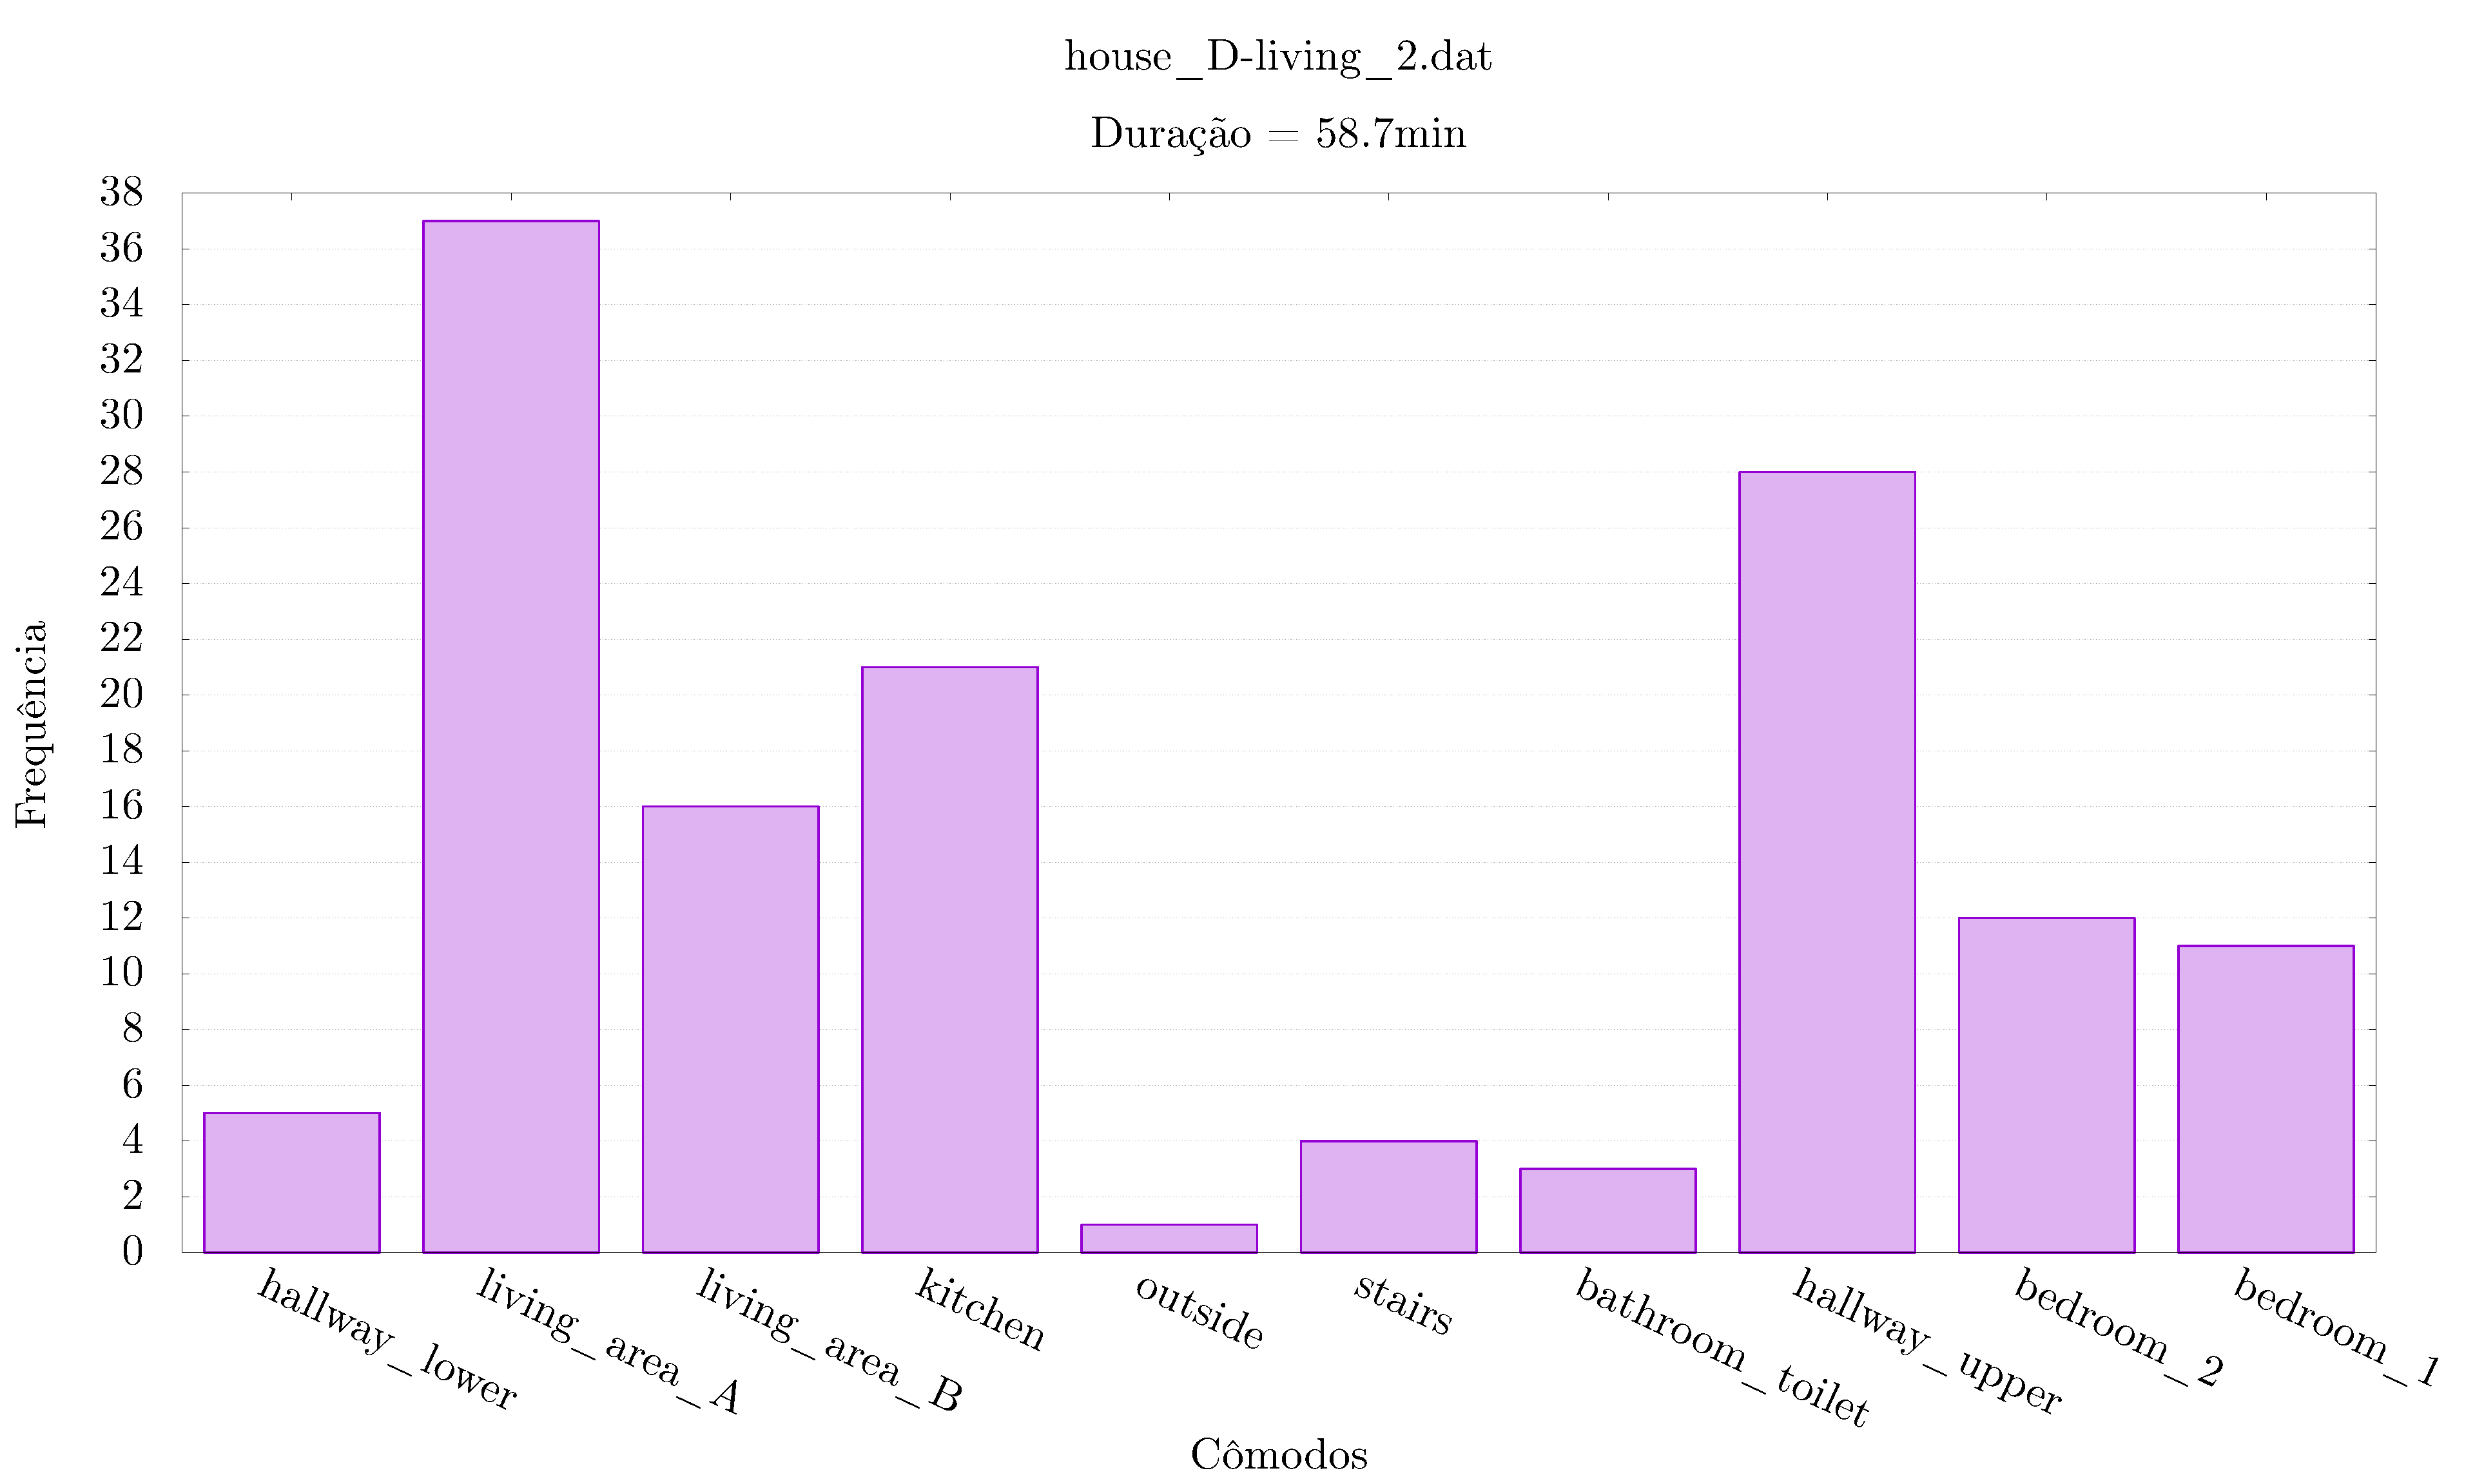
\includegraphics[scale=0.246]{img/dataset-histogram}
		\fonte{\autoriapropria{}}
		
	\end{center}

\end{figure}

O \dataset{} original é composto principalmente por um arquivo de texto que contém em cada linha uma representação de um momento no decorrer do experimento. Entre os dados contidos por linha, destaca-se o \timestamp{} da medição e a etiqueta detectada naquele instante. 

Realizou-se um pré-processamento no \dataset{} de forma a facilitar a utilização dos dados para fim da simulação, gerando um arquivo contendo 3 valores separadas por espaço em que cada linha representa o instante em que o participante entrou e permaneceu contínuamente em um cômodo. Os 3 valores são: um identificador numérico do cômodo, o nome do cômodo e o \timestamp{} em que o indivíduo entrou naquele cômodo, como pode ser visto no \autoref{lst:preprocessed-dataset}.

\begin{center}
	
	\begin{lstlisting}[caption={Parte do \dataset{} pré-processado}, label=lst:preprocessed-dataset]
		#room	room-name	timestamp(seconds)
		2	living_area_A	485.352
		1	hallway_lower	506.273
		6	stairs		513.380
		8	hallway_upper	519.319
		10	bedroom_1	526.159
		8	hallway_upper	561.328
		7	bathroom_toilet	565.832
		8	hallway_upper	628.495
		9	bedroom_2	632.065
	\end{lstlisting}
	
\end{center}

Como descrito anteriormente, cada um dos 10 cômodos possui um \beacon{} \ble{}, configurados para emitir 10 anúncios por segundo. É esperado, então,  que o aplicativo detecte um anúncio a cada 0.1 segundo em que o participante permanece em um cômodo. 

Utilizando o \dataset{} já descrito, a cada momento em que o participante entra em determinado cômodo, calcula-se quantos anúncios o \beacon{} daquele cômodo transmitirá durante o tempo de permanência no local, o cálculo é apresentado a seguir.

\begin{equation}
	anuncios = \frac{tempoPermanencia}{0.1} 
\end{equation}

Onde $tempoPermanencia$ denota o tempo que o indivíduo permaneceu no cômodo. Os anúncios são então repoduzidos a cada intervalo de 0.1 segundo. Com isso foi possível calcular previamente os valores da \autoref{tab:generated-events-1}.

\subsection{Coleta das métricas de performance}

Na \autoref{img:performance-annotation} é possível observar onde os \timestamps{} utilizados na avaliação de performance são anotados. Ambos os \timestamps{} são denotados na imagem por um cronômetro. Na imagem, $T0$ e $T1$ são equivalentes à $TS_{descoberta,\stwopa{}}$ e $TS_{descoberta,app}$ da \autoref{equ:performance-discovery}.

\begin{figure}[htb]
	
	\begin{center}

		\caption{\label{img:performance-annotation}Componentes onde há a captura de \timestamps{}}
		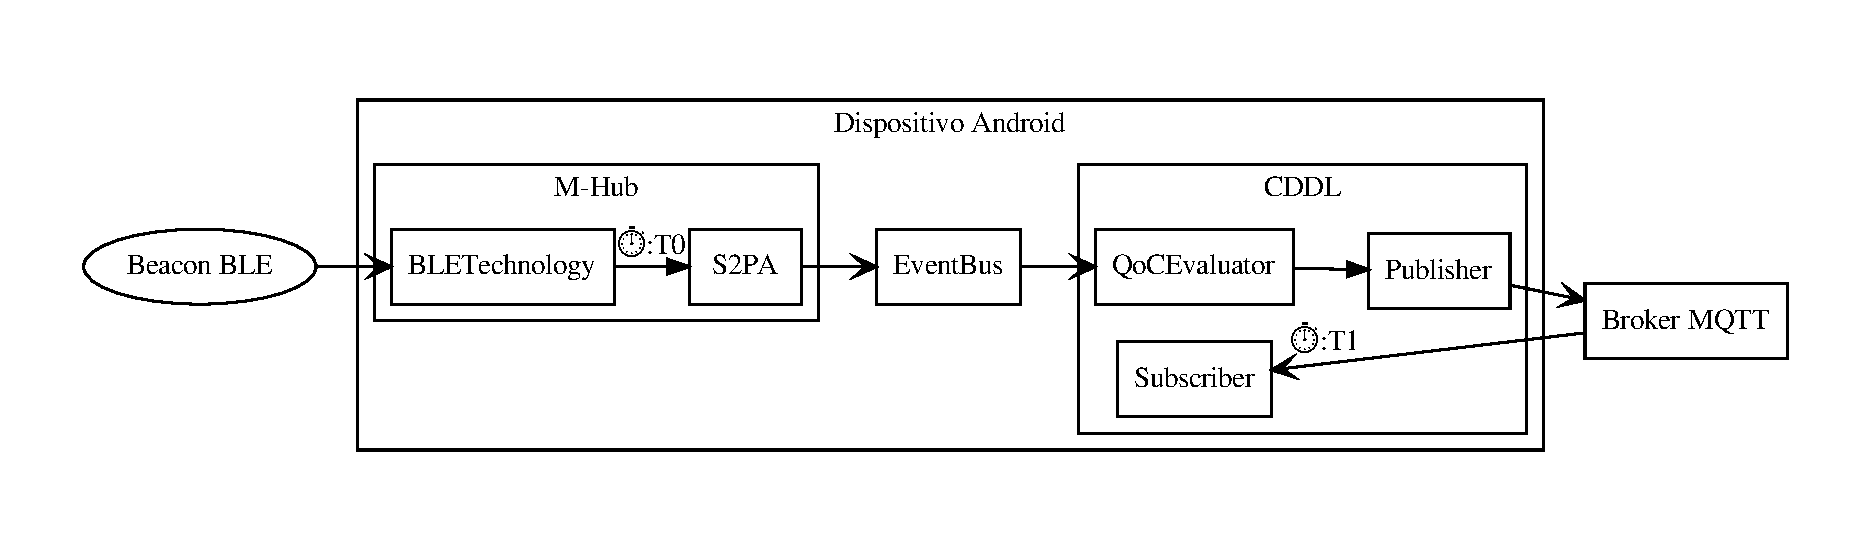
\includegraphics[scale = 0.50]{img/performance-annotation}
		\fonte{\autoriapropria{}}

	\end{center}
	
\end{figure}

\subsection{Recursos computacionais}

O experimento descrito foi executado em um \smartphone{} Lenovo Moto Z Play, com processador de 8 núcleos e 2GHz, e 3GB de memória RAM.

Também foi utilizado uma máquina virtual como \broker{} \mqtt{}, esta máquina executa o sistema operacional Ubuntu 16.04.4 LTS, possui processador de 2 núcleos com 2.5GHz e 4GB de memória RAM.

\section{Experimento 2}

O segundo experimento visa avaliar o desempenho e acurácia da solução proposta, entretanto levando em consideração também os eventos de conexão e desconexão que não foram analisados no primeiro experimento. O experimento consiste em um cenário de uso composto por uma casa equipada com um sistema multimídia na sala de estar que possibilita que \smartphones{} se conectem a ele através de \bluetooth{}, onde o conteúdo da televisão se adapta de acordo com os usuários que estão presentes na sala, e a interação com as aplicações da televisão digital acontece através do \smartphone{}.

O sistema multimídia pode ter ciência de qual usuário está presente através dos \smartphones{} conectados no momento, pois ele armazena a relação dos moradores da residência com seus respectivos \smartphones{}.

Uma aplicação android foi desenvolvida com o \middleware{} \mhubcddl{} que permanece ativamente procurando e se conectando ao sistema multimídia no ambiente. Ao entrar na sala de estar o sistema multimídia é encontrado e em seguida a conexão é estabelecida. Quando o usuário sai da sala de estar a conexão é desfeita. 

\subsection{Métricas}

Para o experimento 2, a todo momento em que o participante entra na sala de estar acontece interações entre o aplicativo e o sistema multimídia, essas interações são compostas de um evento de descoberta, seguido por um evento de conexão. Ao sair do quarto um evento de desconexão é também gerado. Cada um desses eventos são gerados pelo \stwopa{} e notificados posteriormente à aplicação.

As avaliaçãos de desempenho e acurácia deste cenário de uso são análogas às descritas para o experimento 1, com a exceção de que eventos de conexão e desconexão também fazem partes das medições.

A \autoref{equ:performance-discovery} será utilizada para avaliar a performance da notificação de eventos de descoberta. A performance da notificação dos eventos de conexão e desconexão serão os tempos de propagação de tais eventos até a aplicação, e denotados como $TP_{conexao}$ e $TP_{desconexao}$ respectivamente.

\begin{align}
	TP_{conexao} &= TS_{conexao,app} - TS_{conexao,\stwopa{}} \label{equ:performance-connection} \\
	\nonumber\\
	TP_{desconexao} &= TS_{desconexao,app} - TS_{desconexao,\stwopa{}} \label{equ:performance-disconnection}
\end{align}

Onde $TS_{conexao,\stwopa{}}$ e $TS_{desconexao,\stwopa{}}$ são os \timestamps{} de quando os eventos de conexão e desconexão são gerados no \stwopa{}. Já $TS_{conexao,app}$ e $TS_{desconexao,app}$ são os \timestamps{} de quando esses eventos são entregues à aplicação.

Para medir a acurácia será utilizado a \autoref{equ:acuracy}. A \autoref{tab:generated-events-2} sumariza os resultados esperados para o experimento.

\begin{table}[htb]
	\begin{center}
		\IBGEtab{
			\caption{Quantidade de eventos que serão gerados no experimento 2}
			\label{tab:generated-events-2}
		}{
			\begin{tabular}{lc}
				\toprule
				                               & $EventosGerados$ \\
				\midrule 
				\textbf{Eventos de descoberta} & 37               \\
				\textbf{Eventos de conexão}    & 37               \\
				\textbf{Eventos de desconexão} & 37               \\
				\bottomrule
			\end{tabular}
		}{
			\fonte{\autoriapropria}
		}
	\end{center}
\end{table}

\subsection{Simulação do sistema multimídia}

Para este experimento foi feita uma simulação de um indivíduo andando em uma residência, foram utilizados os dados do \dataset{} descrito na \autoref{chap:avaliacao-simulacao-beacons} para esta simulação.

Escolheu-se também o experimento ``\texttt{living\_2}'' da casa ``\texttt{Residence D}'' por fornecer um dos maiores tempos de monitoramento do participante juntamente com a maior quantidade de visitas à sala de estar. Será utilizado apenas a parte do \dataset{} referentes à entradas no cômodo denotado como ``\texttt{living\_area\_A}'' na \autoref{fig:dataset-histogram}, pois este cômodo foi escolhido como a sala de estar onde o sistema multimídia se localiza.

\section{Resultados}

\newcommand{\nullval}{\textbf{---}}

\begin{table}[htb]
	\begin{center}
		\IBGEtab{
			\caption{Quantidade de eventos notificados no experimento 1}
			\label{tab:generated-events-1-results}
		}{
			\begin{tabular}{lccc}
				\toprule
				                               & $EventosGerados$ & $EventosNotificados$ & $Acur\acute{a}cia$ (\%) \\
				\midrule
				\textbf{Eventos de descoberta} & 34814            & 34814                & 100		   \\
				\textbf{Eventos de conexão}    & 0                & 0                    & \nullval	           \\
				\textbf{Eventos de desconexão} & 0                & 0                    & \nullval		   \\
				\bottomrule
			\end{tabular}
		}{
			\fonte{\autoriapropria}
		}
	\end{center}
\end{table}


\begin{table}[htb]
	\begin{center}
		\IBGEtab{
			\caption{Quantidade de eventos notificados no experimento 2}
			\label{tab:generated-events-2-results}
		}{
			\begin{tabular}{lccc}
				\toprule
				                               & $EventosGerados$ & $EventosNotificados$ & $Acur\acute{a}cia$ (\%) \\
				\midrule
				\textbf{Eventos de descoberta} & 37               & 37                   & 100			   \\
				\textbf{Eventos de conexão}    & 37	          & 37                   & 100			   \\
				\textbf{Eventos de desconexão} & 37	          & 37                   & 100			   \\
				\bottomrule
			\end{tabular}
		}{
			\fonte{\autoriapropria}
		}
	\end{center}
\end{table}


%only used in the next table
\newcommand{\tabperformanceheader}{
	& \multicolumn{2}{c}{$TP_{descoberta}$ (ms)} & & \multicolumn{2}{c}{$TP_{conexao}$ (ms)} & & \multicolumn{2}{c}{$TP_{desconexao}$ (ms)} \\
	\cmidrule{2-3} \cmidrule{5-6} \cmidrule{8-9}
	& Média & Desvio padrão                 & & Média & Desvio padrão              & & Média & Desvio padrão                 
}

\begin{table}[htb]
	\begin{center}
		\IBGEtab{
			\caption{Performânce da entrega de mensagens}
			\label{tab:experiments-performance}
		}{
			\scalebox{.97}{
			\begin{tabular}{l*{8}{c}}
				\toprule
				\tabperformanceheader                                                                    \\
				\midrule 
				\textbf{Experimento 1} & 28.03  & 32.71 & & \nullval & \nullval & & \nullval & \nullval \\
				\textbf{Experimento 2} & 77.00 & 29.23  & & 111.11   & 52.74    & & 60.18   & 22.89    \\
				\bottomrule
			\end{tabular}

			}
		}{
			\fonte{\autoriapropria}
		}
	\end{center}
\end{table}

